% Created by tikzDevice version 0.12.6 on 2025-01-28 08:20:29
% !TEX encoding = UTF-8 Unicode
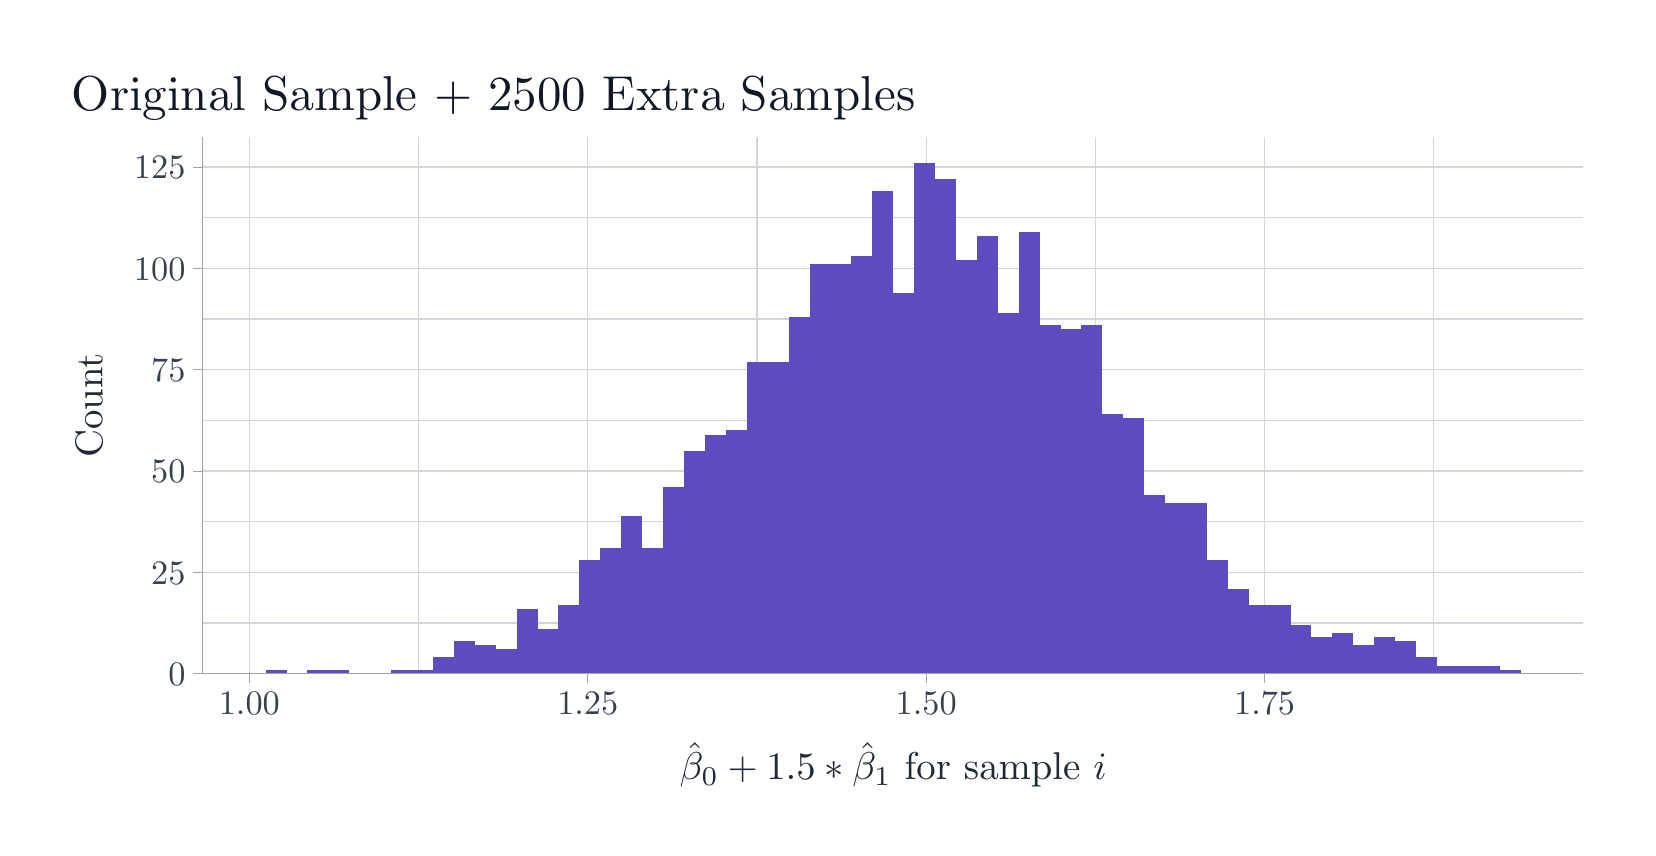
\begin{tikzpicture}[x=1pt,y=1pt]
\definecolor{fillColor}{RGB}{255,255,255}
\path[use as bounding box,fill=fillColor] (0,0) rectangle (578.16,289.08);
\begin{scope}
\path[clip] (  0.00,  0.00) rectangle (578.16,289.08);
\definecolor{drawColor}{RGB}{255,255,255}

\path[draw=drawColor,line width= 0.7pt,line join=round,line cap=round,fill=fillColor] (  0.00,  0.00) rectangle (578.16,289.08);
\end{scope}
\begin{scope}
\path[clip] ( 63.32, 55.65) rectangle (562.16,249.43);
\definecolor{drawColor}{RGB}{255,255,255}
\definecolor{fillColor}{RGB}{255,255,255}

\path[draw=drawColor,line width= 0.7pt,line join=round,line cap=round,fill=fillColor] ( 63.32, 55.65) rectangle (562.16,249.43);
\definecolor{drawColor}{RGB}{209,213,219}

\path[draw=drawColor,line width= 0.4pt,line join=round] ( 63.32, 73.96) --
	(562.16, 73.96);

\path[draw=drawColor,line width= 0.4pt,line join=round] ( 63.32,110.58) --
	(562.16,110.58);

\path[draw=drawColor,line width= 0.4pt,line join=round] ( 63.32,147.19) --
	(562.16,147.19);

\path[draw=drawColor,line width= 0.4pt,line join=round] ( 63.32,183.81) --
	(562.16,183.81);

\path[draw=drawColor,line width= 0.4pt,line join=round] ( 63.32,220.43) --
	(562.16,220.43);

\path[draw=drawColor,line width= 0.4pt,line join=round] (141.24, 55.65) --
	(141.24,249.43);

\path[draw=drawColor,line width= 0.4pt,line join=round] (263.54, 55.65) --
	(263.54,249.43);

\path[draw=drawColor,line width= 0.4pt,line join=round] (385.83, 55.65) --
	(385.83,249.43);

\path[draw=drawColor,line width= 0.4pt,line join=round] (508.12, 55.65) --
	(508.12,249.43);

\path[draw=drawColor,line width= 0.4pt,line join=round] ( 63.32, 55.65) --
	(562.16, 55.65);

\path[draw=drawColor,line width= 0.4pt,line join=round] ( 63.32, 92.27) --
	(562.16, 92.27);

\path[draw=drawColor,line width= 0.4pt,line join=round] ( 63.32,128.89) --
	(562.16,128.89);

\path[draw=drawColor,line width= 0.4pt,line join=round] ( 63.32,165.50) --
	(562.16,165.50);

\path[draw=drawColor,line width= 0.4pt,line join=round] ( 63.32,202.12) --
	(562.16,202.12);

\path[draw=drawColor,line width= 0.4pt,line join=round] ( 63.32,238.74) --
	(562.16,238.74);

\path[draw=drawColor,line width= 0.4pt,line join=round] ( 80.10, 55.65) --
	( 80.10,249.43);

\path[draw=drawColor,line width= 0.4pt,line join=round] (202.39, 55.65) --
	(202.39,249.43);

\path[draw=drawColor,line width= 0.4pt,line join=round] (324.68, 55.65) --
	(324.68,249.43);

\path[draw=drawColor,line width= 0.4pt,line join=round] (446.97, 55.65) --
	(446.97,249.43);
\definecolor{fillColor}{RGB}{92,76,191}

\path[fill=fillColor] ( 85.99, 55.65) rectangle ( 93.55, 57.11);

\path[fill=fillColor] ( 93.55, 55.65) rectangle (101.11, 55.65);

\path[fill=fillColor] (101.11, 55.65) rectangle (108.67, 57.11);

\path[fill=fillColor] (108.67, 55.65) rectangle (116.23, 57.11);

\path[fill=fillColor] (116.23, 55.65) rectangle (123.78, 55.65);

\path[fill=fillColor] (123.78, 55.65) rectangle (131.34, 55.65);

\path[fill=fillColor] (131.34, 55.65) rectangle (138.90, 57.11);

\path[fill=fillColor] (138.90, 55.65) rectangle (146.46, 57.11);

\path[fill=fillColor] (146.46, 55.65) rectangle (154.02, 61.51);

\path[fill=fillColor] (154.02, 55.65) rectangle (161.58, 67.37);

\path[fill=fillColor] (161.58, 55.65) rectangle (169.13, 65.90);

\path[fill=fillColor] (169.13, 55.65) rectangle (176.69, 64.44);

\path[fill=fillColor] (176.69, 55.65) rectangle (184.25, 79.08);

\path[fill=fillColor] (184.25, 55.65) rectangle (191.81, 71.76);

\path[fill=fillColor] (191.81, 55.65) rectangle (199.37, 80.55);

\path[fill=fillColor] (199.37, 55.65) rectangle (206.92, 96.66);

\path[fill=fillColor] (206.92, 55.65) rectangle (214.48,101.06);

\path[fill=fillColor] (214.48, 55.65) rectangle (222.04,112.77);

\path[fill=fillColor] (222.04, 55.65) rectangle (229.60,101.06);

\path[fill=fillColor] (229.60, 55.65) rectangle (237.16,123.03);

\path[fill=fillColor] (237.16, 55.65) rectangle (244.72,136.21);

\path[fill=fillColor] (244.72, 55.65) rectangle (252.27,142.07);

\path[fill=fillColor] (252.27, 55.65) rectangle (259.83,143.53);

\path[fill=fillColor] (259.83, 55.65) rectangle (267.39,168.43);

\path[fill=fillColor] (267.39, 55.65) rectangle (274.95,168.43);

\path[fill=fillColor] (274.95, 55.65) rectangle (282.51,184.54);

\path[fill=fillColor] (282.51, 55.65) rectangle (290.06,203.59);

\path[fill=fillColor] (290.06, 55.65) rectangle (297.62,203.59);

\path[fill=fillColor] (297.62, 55.65) rectangle (305.18,206.52);

\path[fill=fillColor] (305.18, 55.65) rectangle (312.74,229.95);

\path[fill=fillColor] (312.74, 55.65) rectangle (320.30,193.33);

\path[fill=fillColor] (320.30, 55.65) rectangle (327.86,240.20);

\path[fill=fillColor] (327.86, 55.65) rectangle (335.41,234.34);

\path[fill=fillColor] (335.41, 55.65) rectangle (342.97,205.05);

\path[fill=fillColor] (342.97, 55.65) rectangle (350.53,213.84);

\path[fill=fillColor] (350.53, 55.65) rectangle (358.09,186.01);

\path[fill=fillColor] (358.09, 55.65) rectangle (365.65,215.30);

\path[fill=fillColor] (365.65, 55.65) rectangle (373.21,181.61);

\path[fill=fillColor] (373.21, 55.65) rectangle (380.76,180.15);

\path[fill=fillColor] (380.76, 55.65) rectangle (388.32,181.61);

\path[fill=fillColor] (388.32, 55.65) rectangle (395.88,149.39);

\path[fill=fillColor] (395.88, 55.65) rectangle (403.44,147.93);

\path[fill=fillColor] (403.44, 55.65) rectangle (411.00,120.10);

\path[fill=fillColor] (411.00, 55.65) rectangle (418.55,117.17);

\path[fill=fillColor] (418.55, 55.65) rectangle (426.11,117.17);

\path[fill=fillColor] (426.11, 55.65) rectangle (433.67, 96.66);

\path[fill=fillColor] (433.67, 55.65) rectangle (441.23, 86.41);

\path[fill=fillColor] (441.23, 55.65) rectangle (448.79, 80.55);

\path[fill=fillColor] (448.79, 55.65) rectangle (456.35, 80.55);

\path[fill=fillColor] (456.35, 55.65) rectangle (463.90, 73.23);

\path[fill=fillColor] (463.90, 55.65) rectangle (471.46, 68.83);

\path[fill=fillColor] (471.46, 55.65) rectangle (479.02, 70.30);

\path[fill=fillColor] (479.02, 55.65) rectangle (486.58, 65.90);

\path[fill=fillColor] (486.58, 55.65) rectangle (494.14, 68.83);

\path[fill=fillColor] (494.14, 55.65) rectangle (501.69, 67.37);

\path[fill=fillColor] (501.69, 55.65) rectangle (509.25, 61.51);

\path[fill=fillColor] (509.25, 55.65) rectangle (516.81, 58.58);

\path[fill=fillColor] (516.81, 55.65) rectangle (524.37, 58.58);

\path[fill=fillColor] (524.37, 55.65) rectangle (531.93, 58.58);

\path[fill=fillColor] (531.93, 55.65) rectangle (539.49, 57.11);
\end{scope}
\begin{scope}
\path[clip] (  0.00,  0.00) rectangle (578.16,289.08);
\definecolor{drawColor}{RGB}{156,163,175}

\path[draw=drawColor,line width= 0.3pt,line join=round] ( 63.32, 55.65) --
	( 63.32,249.43);
\end{scope}
\begin{scope}
\path[clip] (  0.00,  0.00) rectangle (578.16,289.08);
\definecolor{drawColor}{RGB}{55,65,81}

\node[text=drawColor,anchor=base east,inner sep=0pt, outer sep=0pt, scale=  1.24] at ( 57.02, 51.37) {0};

\node[text=drawColor,anchor=base east,inner sep=0pt, outer sep=0pt, scale=  1.24] at ( 57.02, 87.98) {25};

\node[text=drawColor,anchor=base east,inner sep=0pt, outer sep=0pt, scale=  1.24] at ( 57.02,124.60) {50};

\node[text=drawColor,anchor=base east,inner sep=0pt, outer sep=0pt, scale=  1.24] at ( 57.02,161.22) {75};

\node[text=drawColor,anchor=base east,inner sep=0pt, outer sep=0pt, scale=  1.24] at ( 57.02,197.84) {100};

\node[text=drawColor,anchor=base east,inner sep=0pt, outer sep=0pt, scale=  1.24] at ( 57.02,234.45) {125};
\end{scope}
\begin{scope}
\path[clip] (  0.00,  0.00) rectangle (578.16,289.08);
\definecolor{drawColor}{RGB}{156,163,175}

\path[draw=drawColor,line width= 0.3pt,line join=round] ( 59.82, 55.65) --
	( 63.32, 55.65);

\path[draw=drawColor,line width= 0.3pt,line join=round] ( 59.82, 92.27) --
	( 63.32, 92.27);

\path[draw=drawColor,line width= 0.3pt,line join=round] ( 59.82,128.89) --
	( 63.32,128.89);

\path[draw=drawColor,line width= 0.3pt,line join=round] ( 59.82,165.50) --
	( 63.32,165.50);

\path[draw=drawColor,line width= 0.3pt,line join=round] ( 59.82,202.12) --
	( 63.32,202.12);

\path[draw=drawColor,line width= 0.3pt,line join=round] ( 59.82,238.74) --
	( 63.32,238.74);
\end{scope}
\begin{scope}
\path[clip] (  0.00,  0.00) rectangle (578.16,289.08);
\definecolor{drawColor}{RGB}{156,163,175}

\path[draw=drawColor,line width= 0.3pt,line join=round] ( 63.32, 55.65) --
	(562.16, 55.65);
\end{scope}
\begin{scope}
\path[clip] (  0.00,  0.00) rectangle (578.16,289.08);
\definecolor{drawColor}{RGB}{156,163,175}

\path[draw=drawColor,line width= 0.3pt,line join=round] ( 80.10, 52.15) --
	( 80.10, 55.65);

\path[draw=drawColor,line width= 0.3pt,line join=round] (202.39, 52.15) --
	(202.39, 55.65);

\path[draw=drawColor,line width= 0.3pt,line join=round] (324.68, 52.15) --
	(324.68, 55.65);

\path[draw=drawColor,line width= 0.3pt,line join=round] (446.97, 52.15) --
	(446.97, 55.65);
\end{scope}
\begin{scope}
\path[clip] (  0.00,  0.00) rectangle (578.16,289.08);
\definecolor{drawColor}{RGB}{55,65,81}

\node[text=drawColor,anchor=base,inner sep=0pt, outer sep=0pt, scale=  1.24] at ( 80.10, 40.78) {1.00};

\node[text=drawColor,anchor=base,inner sep=0pt, outer sep=0pt, scale=  1.24] at (202.39, 40.78) {1.25};

\node[text=drawColor,anchor=base,inner sep=0pt, outer sep=0pt, scale=  1.24] at (324.68, 40.78) {1.50};

\node[text=drawColor,anchor=base,inner sep=0pt, outer sep=0pt, scale=  1.24] at (446.97, 40.78) {1.75};
\end{scope}
\begin{scope}
\path[clip] (  0.00,  0.00) rectangle (578.16,289.08);
\definecolor{drawColor}{RGB}{31,41,55}

\node[text=drawColor,anchor=base,inner sep=0pt, outer sep=0pt, scale=  1.40] at (312.74, 17.36) {$\hat{\beta}_0 + 1.5 * \hat{\beta}_1$ for sample $i$};
\end{scope}
\begin{scope}
\path[clip] (  0.00,  0.00) rectangle (578.16,289.08);
\definecolor{drawColor}{RGB}{31,41,55}

\node[text=drawColor,rotate= 90.00,anchor=base,inner sep=0pt, outer sep=0pt, scale=  1.40] at ( 27.00,152.54) {Count};
\end{scope}
\begin{scope}
\path[clip] (  0.00,  0.00) rectangle (578.16,289.08);
\definecolor{drawColor}{RGB}{17,24,39}

\node[text=drawColor,anchor=base west,inner sep=0pt, outer sep=0pt, scale=  1.77] at ( 16.00,259.15) {Original Sample + 2500 Extra Samples};
\end{scope}
\end{tikzpicture}
